\section{Durchführung}

\subsection{Lichtführung}

Verwendet wird eine Quecksilberlampe, die nur bestimmte Wellenlängen emmitiert. Dieses wird zunächst durch eine Linse
auf einen Einzelspalt gestreut. Durch die Breite des Spalts kann dann die breite der Linien der verschiedenen Wellenlängen 
variiert werden. Dabei wird allerdings auch die Intensität des Lichts verringert.\\
\noindent Danach wird das Licht wieder durch eine weitere Linse gebündelt werden. Die Linsen sollten so platziert sein, sodass
das Linienbild des Lichts am Ende scharf aussieht. Das gebündelte Licht wird zunächst jedoch noch durch ein Prisma
geschickt, um die verschiedenen Wellenlängen voneinander zu trennen. 

\begin{figure}[H]
    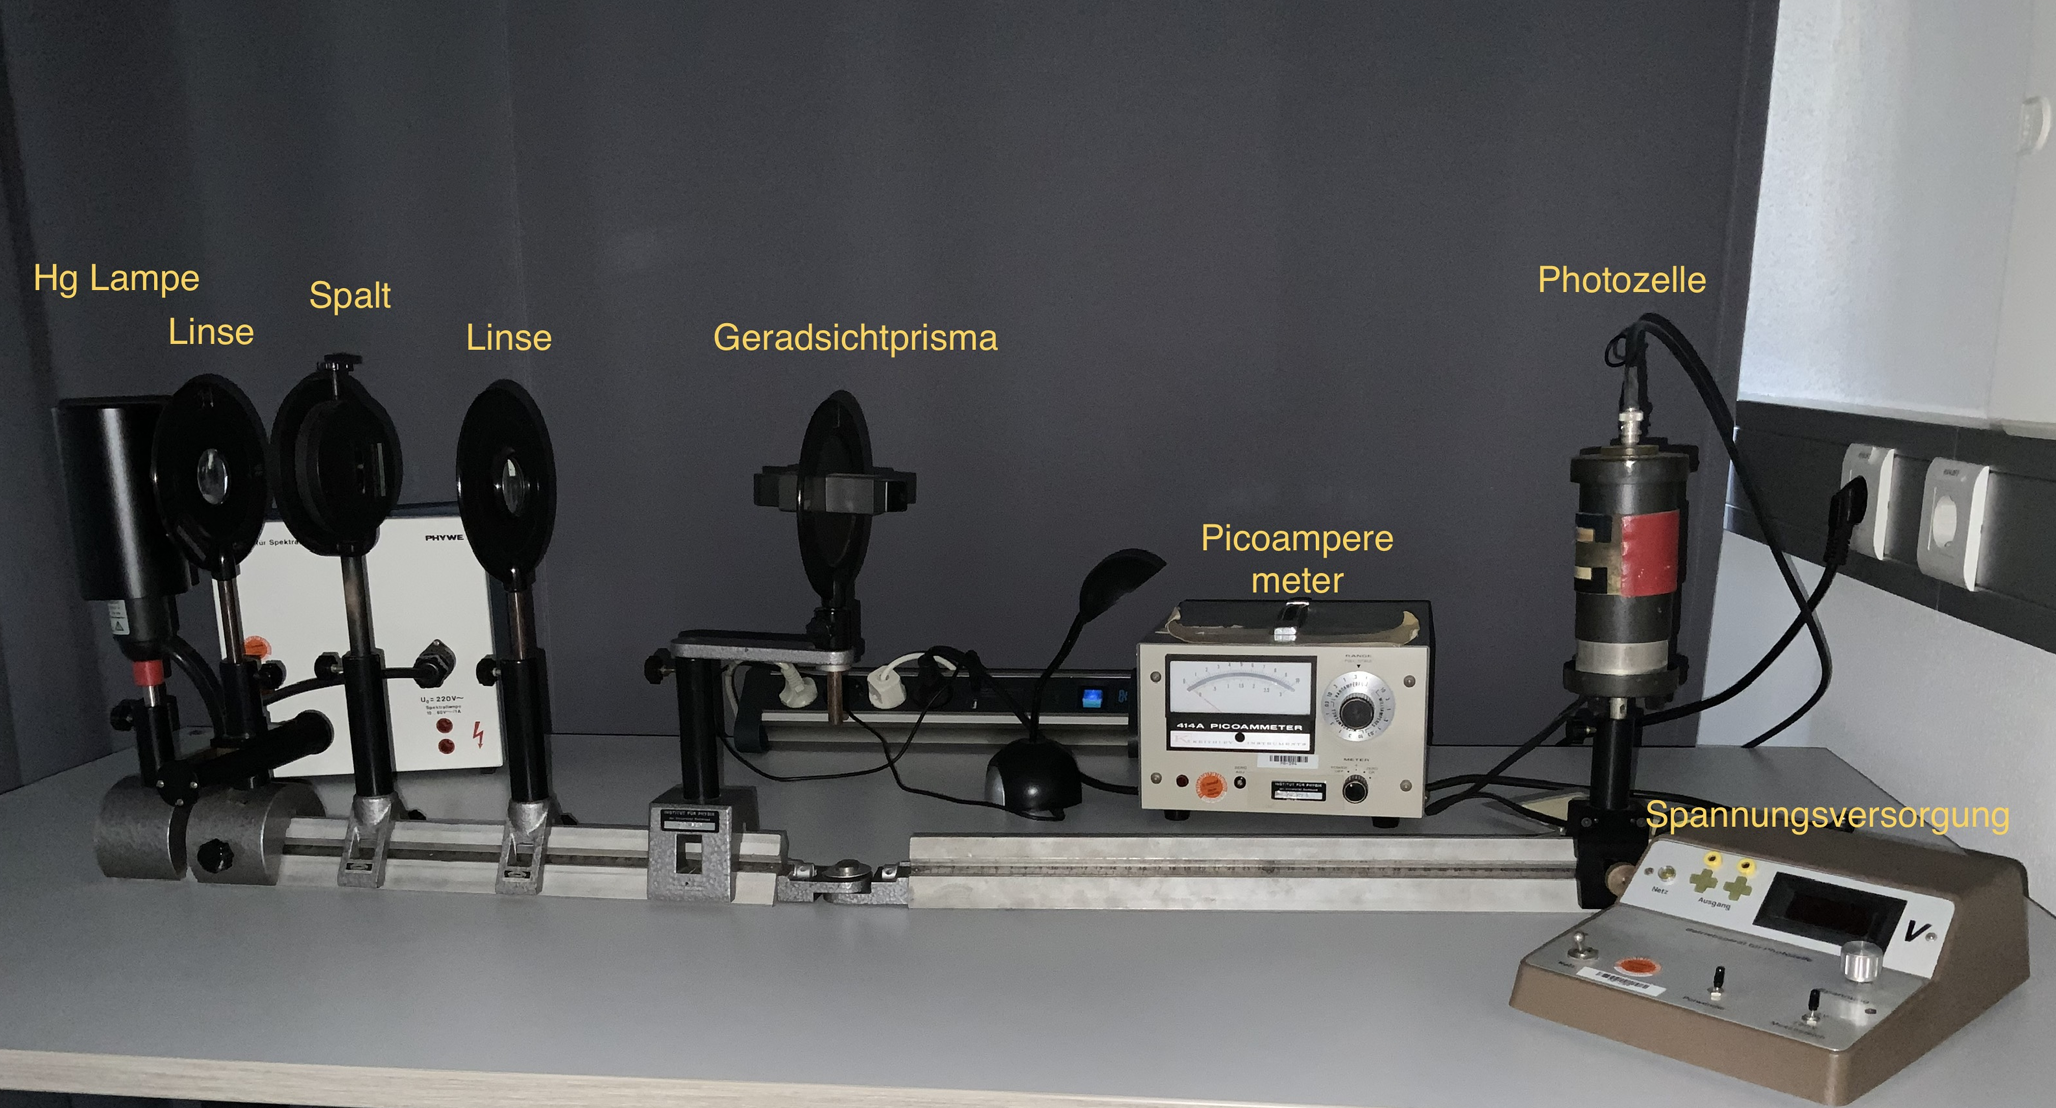
\includegraphics[width=\textwidth]{Bilder/Aufbau.png}
    \caption{Aufbau des Versuchs.}
\end{figure}

\subsection{Durchführung}

Als erstes wird der Fokus auf eine bestimmte Wellenlänge gelegt, hier $\lambda=\qty{435.8}{\nano\meter}$. 
Dazu wird zunächst die Grenzspannung $U_G$ von dem Gegenfeld gemessen, ab der das Strommessgerät anfängt auszuschlagen.
Danach wird diese Spannung jeweils um $\qty{50}{\milli\volt}$ verringert und die Photostromstärke aufgezeichnet.
Nach einiger Zeit werden diese Schritte dann auf bis zu $\qty{1}{Volt}$ erhöht und wenn nötig umgepolt und weiter der 
Strom gemessen. Die großschrittige Messung wird dann bei etwa halber Lichtintensität wiederholt.\\
Als letztes wird die kleinschrittige Messung dann für weitere Wellenlängen wiederholt, wobei die Linien auf dem Schirm
dabei nicht überlappen dürfen.